
\chapter{Methodology} \label{chap_3}
\ \\
The objective of this thesis was to see if there were any overlooked bugs in common fuzzing benchmarks, choosing OSS-Fuzz and FuzzBench as they are among the most popular ones. This, in turn, meant analyzing the effectiveness of such automated testing campaigns and verify how efficiently they were being employed by open-source developers.

What does it mean for a bug to be "overlooked" in this context?

If we think about OSS-Fuzz, where fuzzing is performed automatically by VMs, it means to look for cases where machines failed: this could happen either due to a fault in the automation process or due to the integration choices made by the developers. In the first case, we may talk about limits imposed by OSS-Fuzz on its resources, like tests that cause out-of-memory scenarios, timeouts or even bugs that cannot be reliably and consistently reproduced.  In the second case, it is strictly related to the content of the \textit{project.yaml} configuration file: different sanitizers look for different types of bugs, while each fuzzing engine uses its own set of strategies to test a program, producing results that may be completely different from the other provided fuzzers. For this reason, I focused on the latest public "fuzzing queue" made available by the developers, i.e. the corpus of inputs used by OSS-Fuzz when performing the tests.

If we think about FuzzBench, where projects are actively tested by several different fuzzers, it means to look for bugs discovered in older versions that were not tested on newer ones, which obviously is a human error. A small selection of projects from OSS-Fuzz are tested continuously by several different fuzzers, producing daily reports available both to the fuzzers and the chosen projects developers, along with public access to the corpora used to perform the tests as well as the results and the crashes found (if any). It is then responsibility of the project developers to analyze and fix these bugs, although this does not always happen. For this reason, I focused on analyzing a chosen set of experiments between 2020 and 2024, downloading all the available crashes and testing them on latest version, hoping to find old bugs that have yet to be fixed.

As previously mentioned, all relevant bugs were then appropriately reported to their respective developers.



\newpage
\section{Setting up the environment}
All tests were performed on two separate machines, both equipped with personal installations of Ubuntu 22.04 LTS, already run-in and used.


Regarding tools for general purpose, I used Docker, Valgrind, Python 3, gsutil and Google Chrome.

The \textit{Docker} \cite{Docker} application run the different containers needed by OSS-Fuzz to build the environment where projects will be built and tested.

\textit{Valgrind} \cite{Valgrind_1}\cite{Valgrind_2} is a dynamic binary instrumentation (DBI) framework to perform analysis, profiling and management of a program during its execution.
More specifically, it was used to perform memory analysis when projects were built without sanitizers.

The \textit{Python 3} language was used to create several scripts that I used to perform information scraping, reports analysis and bug deduplication.
It is also used by OSS-Fuzz to provide some functionalities, and this will be discussed later. 

The \textit{gsutil} suite is a command-line tool provided by Google to access resources stored on Google Cloud Service from your local machine, and it was used to analyze the FuzzBench benchmarks and download other resources.

Finally, \textit{Google Chrome} and its "development driver" were needed during the information scraping phase of this work, discussed in section \ref{selection}.


Regarding \textit{OSS-Fuzz}, most of the work was done on its GitHub repository, which I cloned locally on both machines.
To provide its services, OSS-Fuzz uses several python scripts that can be invoked via command-line using appropriate arguments. These commands can be used to update the projects' files and projects' images, build the project's image and its fuzzers but also download resources like corpora. 


Regarding \textit{FuzzBench}, most of the work was done on its Google Cloud bucket, specifically on the section where all experiments results are collected.
To access and later download the resources needed, I incorporated the \textit{gsutil} suite in a python script to perform web scraping.

\newpage
\section{OSS-Fuzz}
\subsection{Selecting the projects} \label{selection}
At the moment of writing, the OSS-Fuzz campaign includes over 1000 projects that are actively fuzzed and tested, but it would obviously be impossible to rebuild and test all of them locally also due to the language heterogeneity of such projects.

For this reason, this work focused solely on projects using the C/C++ language.

Then, to further narrow down the analysis, I identified 5 different categories of projects using the number of sanitizers used by the developers, keeping ASan as the reference due to its popularity and efficiency.

Finally, I ordered each set by "highest number of bugs issued" using the OSS-Fuzz bug tracker and tested these lists top-down until I had 5 projects for each category that were building and fuzzing correctly.
\ \\ 
 

First step in this process was to extract the list of all projects written in C/C++, and this was done by performing a preliminary analysis of the \textit{project.yaml} configuration file present inside each project's directory.
\newline
\begin{figure}[h]
\centering
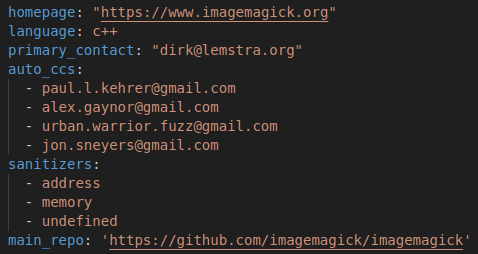
\includegraphics[scale=0.65]{foto/project_yaml.png}
\caption{Example of content from a project.yaml}
\label{fig:project_yaml}
\end{figure}
\ \\
To retrieve the language used by each project, I initially wrote a simple Python script taking as input the OSS-Fuzz "project" directory.

Then, the script opened the directory list of the argument provided and iteratively explored each project's directory looking for the aforementioned configuration file: assuming the file was found, it then opened the file and scanned each line looking for the "language: c" string, eventually saving the name of such projects in a list.
This yielded a total of 524 projects out of 1277 written using C/C++.

To perform the categorization of the projects depending on the number of sanitizers used, I extended the previous script to also look for the strings "address", "memory" and "undefined", shown on image \ref{fig:project_yaml}.

The assignment uses a binary logic on decimal values, starting each project from 0 and giving each sanitizer a different value (1, 10, 100), so that by summing them I could easily understand which sanitizers were found in its configuration file.
Out of the previous 524 projects, the results were as follows: 238 used all sanitizers, 22 used ASan and MSan, 62 used ASan and UBSan, 46 used only ASan and 156 did not use any sanitizers.
\ \\ 
 

The next step was retrieving the number of discovered bugs of each project, and this required a thorough analysis of the "OSS-Fuzz Issue Tracker" website. \cite{ossfuzz_bugtracker}

\begin{figure}[h]
\makebox[\textwidth][c]{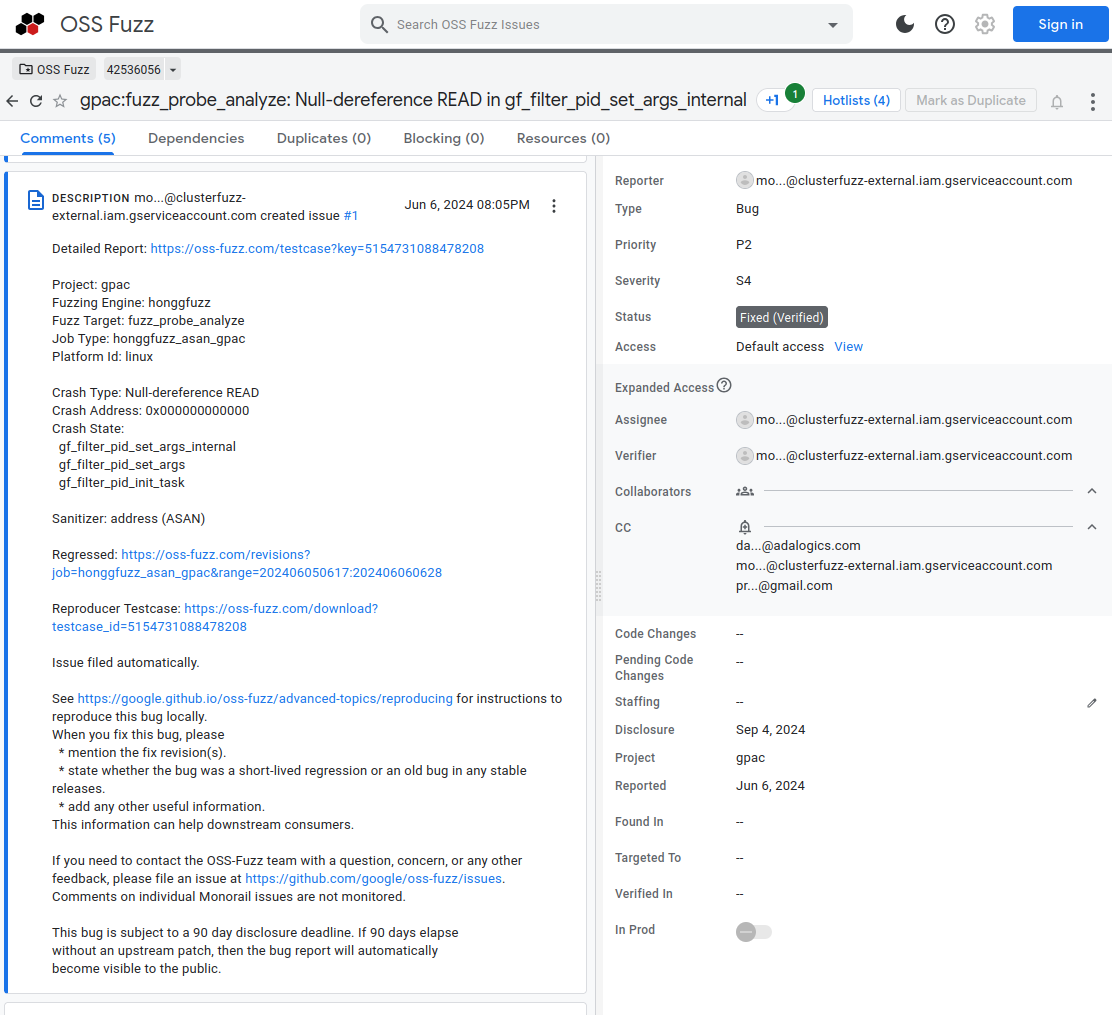
\includegraphics[width=0.69\paperwidth]{foto/issue.png}}
\caption{Example of bug report \cite{ossfuzz_bugtracker}}
\label{fig:issue}
\end{figure}
\ \\
At the moment of writing, the issue tracker platform was changed from "Monorail" to "Google Sites", so most of the work described here may no longer work as intended.



Given that Monorail APIs could only be used by projects' developers registered to OSS-Fuzz and that there weren't any files that could be used for an offline analysis, I had to perform website scraping on the individual issues to retrieve the information. 

To do this, I used as reference a GitHub repository written by Zhen Yu Ding called "Monorail Scraper" \cite{scraper}, a tool to scrape and retrieve data from Monorail, that also included functionalities for ClusterFuzz-generated OSS-Fuzz issues.
The tool relies on the Google Chrome web browser and their testing development tool called "ChromeDriver" \cite{driver}: this is an autonomous web server implementing "W3C WebDriver" \cite{driver_standard}, a standard providing a remote interface to control user-agents and a set of interfaces to perform analysis and manipulation of DOM elements.

Essentially, this allows the user to write scripts that, in turn, instruct the Google Chrome browser to visit a specific web page and possibly performs some interaction with it, like pushing a button, compiling a form or visiting another webpage by exploring the DOM elements.  
In this work, I focused on the functionalities for the analysis of OSS-Fuzz reports.

Initially, the user provides a range of "report IDs" to retrieve.

Then, the tool opens a new Google Chrome instance and performs a connection to a specific link in the Monorail website, attempting the reconnection only once if the first one fails. If the resulting DOM shows a login form, it means that the requested bug is still in the disclosure window, in which case the next ID is analyzed.

Assuming that the requested report is publicly accessible, the DOM is scanned for key information.
During this phase, given that the project is already few years old, I had to make some minor corrections and adjustments as some parameters collected were changed and/or missing altogether.

All the information collected by each report was then stored in JSON files.

\begin{figure}[h]
\makebox[\textwidth][c]{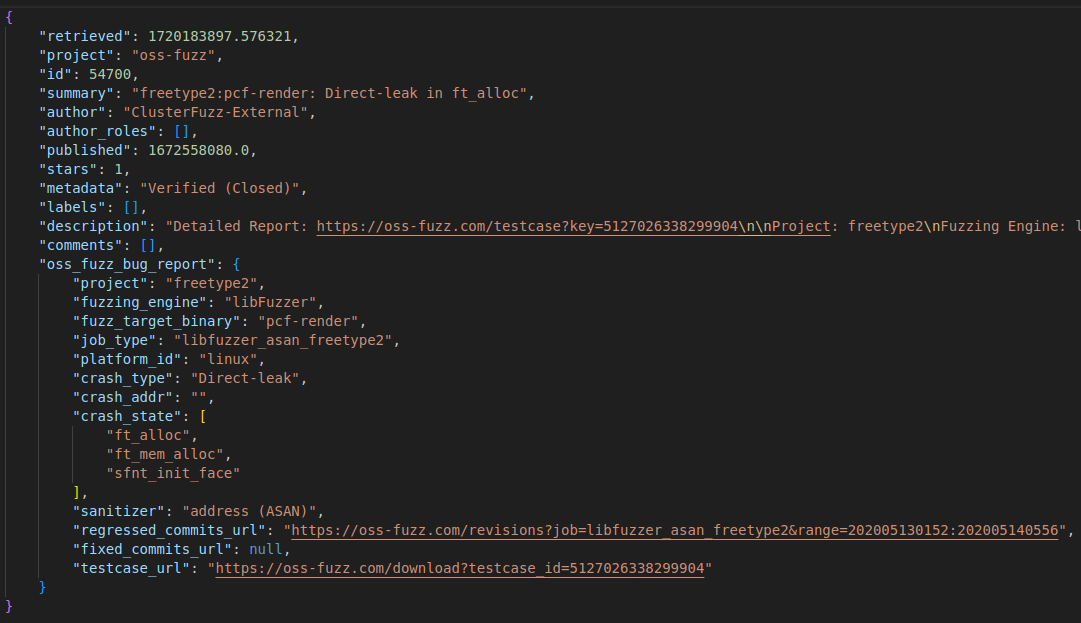
\includegraphics[width=0.66\paperwidth]{foto/json.png}}
\caption{Example of information collected from reports in JSON}
\label{fig:report}
\end{figure}
\ \\
The analysis was performed on all bugs between 2023-01-01 and 2024-06-31, for a total of 11743 collected reports.


The second to last step was to analyze the previously obtained JSON files and make a list of the most bugged projects for each category.

To do this, I initially wrote a simple Python script that takes as input the JSON files and analyzes the information fields collected.

First, I checked the \textit{"metadata"} field for values like "WontFix", "Duplicate" or "Invalid": the first means that the developers themselves tagged that specific bug as non-relevant and will not be addressed in the future, the second refers to a report for a bug that has been already issued but triggered by a different testcase, while the last one means that the reported bug could not be reliably reproduced.

Then, I checked the \textit{"description"} field for manual reports, as they were not meaningful towards the final results. 

Assuming the report analyzed is valid and generated by ClusterFuzz, I retrieved the project name from the \textit{"oss\_fuzz\_bug\_report"} fields and used a dictionary key-value to keep track of the number of bugs reported for each project. 

\begin{figure}[h]
\centering
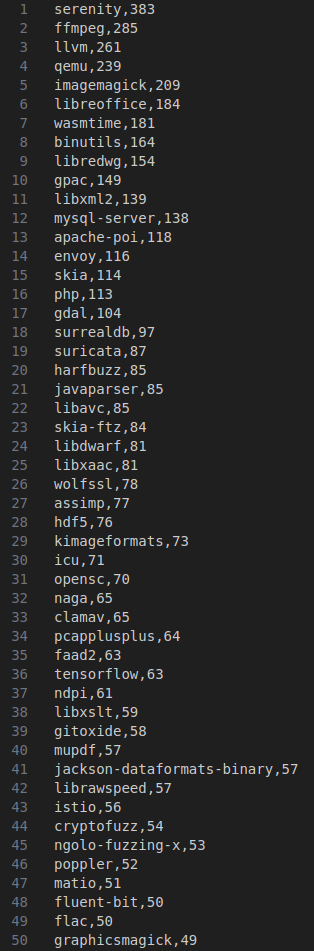
\includegraphics[scale=0.44]{foto/list.png}
\caption{Excerpt of the 50 most bugged projects}
\label{fig:list}
\end{figure}

The last step was to analyze each project individually and determine which harness produced the highest number of reports.

Given the previous script, I extended it to take as input also a project name, so that the parsing of the JSON file focused only on reports for that particular project, and the dictionary key-value was now used to keep track of the number of bugs produced by each fuzzing target binary.
\ \\ 
 

All this resulted in the following projects and harnesses being tested:
\begin{itemize}
  \item \textbf{All Sanitizers}
  \begin{itemize}
    \item binutils (fuzz\_objdump\_safe)
    \item harfbuzz (hb-subset-fuzzer)
    \item imagemagick (encoder\_heic\_fuzzer)
    \item libxml2 (valid)
    \item skia (skruntimeeffect)
  \end{itemize}
  \item \textbf{ASan + MSan}
  \begin{itemize}
    \item ghostscript (gs\_device\_pdfwrite\_fuzzer)
    \item libyang (lyd\_parse\_mem\_json)
    \item wasmedge (wasmedge-fuzztool)
    \item openjpeg (opj\_decompress\_fuzz\_J2K)
    \item myanmar-tools (zawgyi\_detector\_fuzz\_target)
  \end{itemize}
  \item \textbf{ASan + UBSan}
  \begin{itemize}
    \item cairo (svg-render-fuzzer)
    \item clamav (clamav\_dbload\_YARA\_fuzzer)
    \item freerdp (TestFuzzCoreClient)
    \item tarantool (luaL\_loadbuffer\_fuzzer)
    \item vlc (vlc-demux-dec-libfuzzer)
  \end{itemize}
  \item \textbf{ASan only}
  \begin{itemize}
    \item fwupd (uswid\_fuzzer)
    \item glslang (compile\_fuzzer)
    \item inchi (inchi\_input\_fuzzer)
    \item radare2 (ia\_fuzz)
    \item zeek (zeek-ftp-fuzzer)
  \end{itemize}
  \item \textbf{No Sanitizers}
  \begin{itemize}
    \item fluent-bit (flb-it-fuzz-cmetric\_decode\_fuzz\_OSSFUZZ)
    \item gpac (fuzz\_probe\_analyze)
    \item libdwarf (fuzz\_debug\_str)
    \item libredwg (llvmfuzz)
    \item serenity (FuzzJs)
  \end{itemize}
\end{itemize}





\subsection{Testing with OSS-Fuzz}
The OSS-Fuzz repository contains several tools to build and test the available projects, as well as debugging and reproduction scripts.

Most of the tools used in this work are provided by the "helper.py" script, which I used to download a project's Docker image, build the fuzzers and download the public corpora made available by the developers.
The commands used are:
\begin{verbatim}
    $ python3 helper.py pull_images 

    $ python3 helper.py build_image {project_name}

    $ python3 helper.py build_fuzzers {project_name}
        --sanitizer={address(default),memory,undefined,none} 
            --engine={libfuzzer(default),afl, honggfuzz, centipede}
        
    $ python3 helper.py download_corpora 
        --project={project_name} --fuzz-target={harness_name}
\end{verbatim}
\ \\
The \verb|pull_images| argument connects to OSS-Fuzz's Google Bucket to download and update all the Docker "base images" on your local machine, which are used by all projects as the base image to create their respective testing environment.
The \verb|build_image| argument takes as input the name of a project and builds its Dockerfile, creating a new image on your local machine that will be later used to perform fuzzing. During this process, all dependencies and resources needed to correctly compile the fuzzers are downloaded and installed, including the main \textit{build.sh} script. It was used in conjunction with daily \verb|git pull| on the OSS-Fuzz repository, to make sure that I was always building the latest version. 
The \verb|build_fuzzers| argument takes as input the name of a project and a list of possible sanitizers and fuzzing engines to be used during the compilation of the fuzz targets. Although this command accepts only one sanitizer at a time, it's possible to mix them by acting on some environment variables provided by the base images. Finally, this script acts as a "wrapper" for a much more complex Docker command, that creates the project's Docker image using some specific environment variables and invokes the execution of the \textit{build.sh} script.
The \verb|download_corpora| argument takes as input a project name and a fuzz target, it then connects to the project's Google Bucket and downloads the latest public corpus for the provided fuzz target.
After executing these commands, three new directories are created.

The \verb|out| directory contained the project's directory where all built files were saved, including libraries, fuzz targets and other files created by the selected fuzzer.

The \verb|work| directory acted as a temporary location to store intermediate files during the building process and the fuzzing sessions.

The \verb|corpus| directory contained the downloaded corpora stored as zip files.


To prepare the tests, I was tasked with building the chosen harnesses using all possible values for sanitizers, meaning that each project was compiled 4 times: with ASan only, with MSan only, with UBSan only and without any sanitizer.

Moreover, all projects were built using AFL as fuzzing engine, as it is the current state-of-the-art fuzzer. 
The tests were performed inside each project's Docker image, created and configured using the following command:
\begin{verbatim}
    $ docker run --rm --privileged --platform linux/amd64 
        -v /oss-fuzz/build/out/{project_name}/:/out/
        -v /oss-fuzz/build/corpus/{project_name}/:/corpus/    
        -v /home/zio-saba/Scrivania/TESI/logfiles/:/logfiles/ 
        -it  gcr.io/oss-fuzz/{project_name} /bin/bash
\end{verbatim}
\ \\
This is a shorter and modified version of the command invoked by the \verb|build_fuzzer| wrapper.
The first few parameters are needed to create a privileged instance of Docker and specify the running platform on which the fuzz targets will be tested.
The arguments starting with \verb|-v| are used to create a shared directory in the Docker container, which means linking a local directory to a virtual one created inside the container. This was needed to make sure that I could access the resources stored locally on my machine (i.e. fuzz targets, libraries and their corpus) from inside the Docker container used for the tests.
The last line invokes the project image to load as well as making it interactive by spawning a \verb|/bin/bash| process.

 
 
 

Once the Docker images has been loaded and ready to use, some final adjustments were performed to perform the tests.
All tests performed on fuzz targets built with MSan required the sanitizer's libraries to be copied in some specific locations, using the following commands:
\begin{verbatim}
    $ cp -R /usr/msan/lib/* /usr/local/lib/x86_64-unknown-linux-gnu/
    $ cp -R /usr/msan/include/* /usr/local/include
\end{verbatim}
\ \\
All tests performed on fuzz targets built without sanitizers relied on Valgrind to perform binary analysis and profiling, installed using the following command:\begin{verbatim}
    $ sudo apt install gdb valgrind
\end{verbatim}
\ \\
Sometimes, the \verb|apt| tool was not available in a specific Docker container: this is because all base images provided by OSS-Fuzz contain a minimal installation of Linux Ubuntu with only some key packages that are usually enough to compile a programs, such as compiler, assembler, text editors and standard libraries.

In such cases, the \verb|unminimize| command was executed, which essentially "unpacks" the container and reverts it to a standard Ubuntu image, reinstalling all the default packages as well as standard additional tools.

\newpage
When testing fuzz targets built with ASan, MSan or UBSan, I used the following command:
\begin{verbatim}
    $ for i in /corpus/*; do 
        echo "TEST" $i; 
        echo "TEST" $i >> /logfiles/PROJECT_SANITIZER-NAME.log; 
        ./{fuzz_target} $i &>> /logfiles/PROJECT_SANITIZER-NAME.log; 
      done
\end{verbatim}
\ \\
This commands uses the shell \verb|for| construct to scan all files found in the "corpus" directory.

Then, it prints the name of the current testcase on the terminal, which I used for monitoring purposes.

Finally, it prints the name of the current testcase and the results of the fuzz target executed on that particular testcase on a log file.

\begin{figure}[h]
\makebox[\textwidth][c]{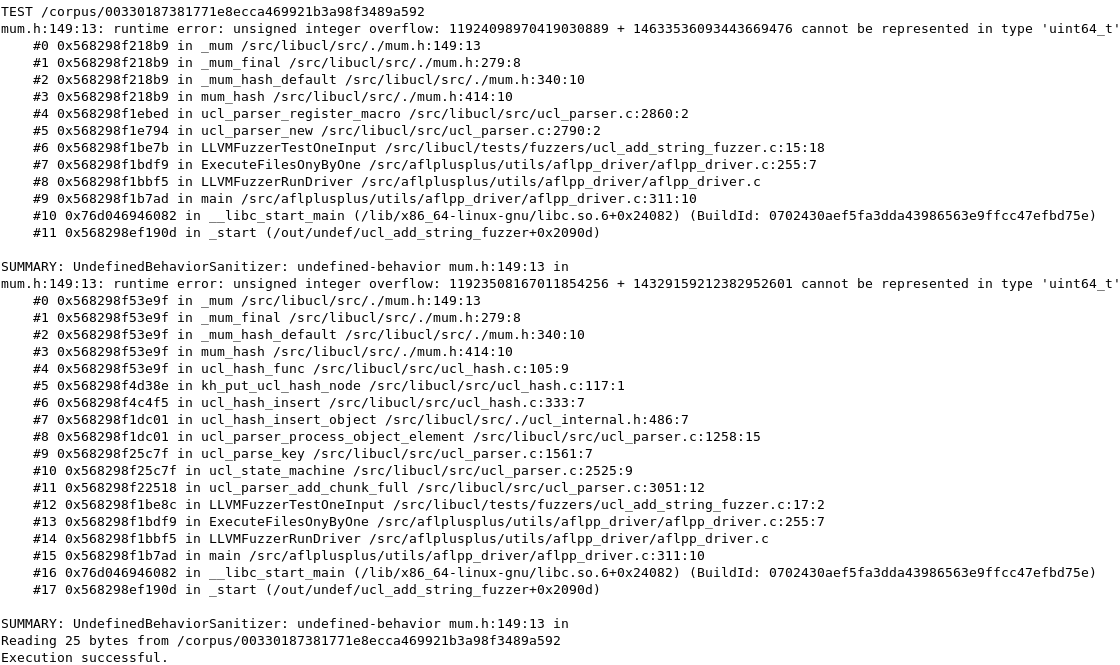
\includegraphics[width=0.8\paperwidth]{foto/ubsan_example.png}}
\caption{Example of integer-overflow bug reported by UBSan}
\label{fig:ubsan_example}
\end{figure}
\ \\

\newpage
When testing fuzz targets built without any sanitizers, I used Valgrind to analyze and profile the binary's execution, using the following command:
\begin{verbatim}
    $ for i in /corpus/*; do 
        echo "TEST" $i; 
        valgrind --log-fd=9 9>>/logfiles/PROJECT_valgrind.log 
            ./{fuzz_target} $i >> /logfiles/PROJECT_valgrind.log 
            && echo -e "\n\n" >> /logfiles/PROJECT_valgrind.log; 
      done
\end{verbatim}
\ \\
Again, I used the shell \verb|for| construct to scan all files found in the "corpus" directory and print the name of the current testcase on the terminal for monitoring purposes.

Then, I invoked Valgrind with a custom file descriptor, which allowed me to capture \verb|STDERR| and print it in the log file.

Finally, it prints the result of the fuzz target executed on that particular testcase on a log file.

\begin{figure}[h]
\makebox[\textwidth][c]{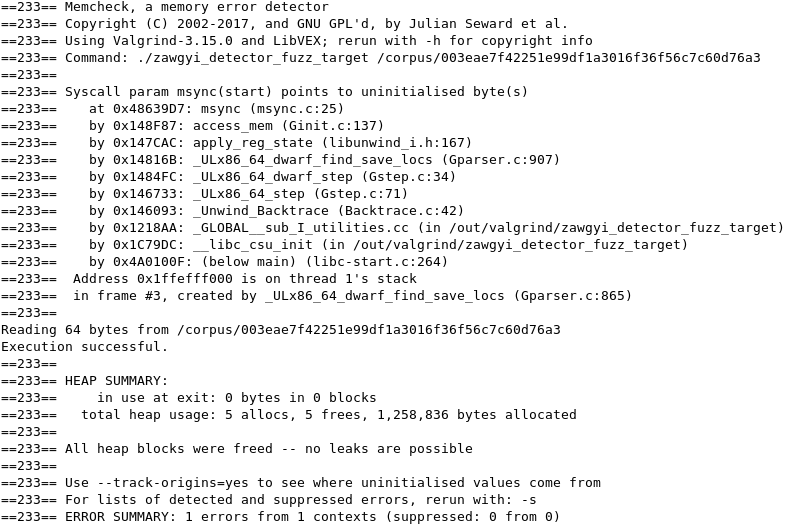
\includegraphics[width=0.65\paperwidth]{foto/valgrind_example.png}}
\caption{Example of use-of-uninitialized-memory (UUM) bug reported by Valgrind}
\label{fig:valgrind_example}
\end{figure}
\ \\


\newpage
However, not all projects built on their first attempt.
In most cases, the building process failed due to missing libraries: for example, libraries like \verb|pthread| and \verb|math| were often automatically added by the sanitizers.

Other times, libraries were not being correctly linked and/or were missing crucial compiling flags, like \verb|-ldl| and \verb|-lz|.
To fix these problems, I had to manually modify the source files and compile the fuzz targets from inside the Docker container, using a command similar to the one executed by \verb|compile_fuzzers|:
\begin{verbatim}
    $ docker run --rm --privileged --platform linux/amd64 
        -e PROJECT_NAME={project_name} -e HELPER=True 
        -e FUZZING_LANGUAGE=c++ 
        -e FUZZING_ENGINE=afl 
        -e SANITIZER={address,memory,undefined,none} 
        -v /oss-fuzz/build/out/{project_name}/:/out/   
        -v /oss-fuzz/build/work/{project_name}/:/work/
        -it  gcr.io/oss-fuzz/{project_name} /bin/bash
\end{verbatim}
\ \\
Similarly to before, the first few parameters are needed to create a privileged instance of Docker and specify the running platform on which the fuzz targets will be tested, the arguments starting with \verb|-v| are used to create a shared directory in the Docker container and the last line invokes the project image to load as well as making it interactive by spawning a \verb|/bin/bash| process.
The novelty lies in the arguments starting with \verb|-e|, which can be used to override the environment variables provided by the Docker image.

These variables can be used by the source files to compile a program using the most appropriate compile flags, fuzzing engine and sanitizers, and they can be easily modified by the user when creating the Docker image to easily re-target the compilation with little to none effort.
After loading the Docker image and modifying the source files, the command \verb|compile| invokes the execution of the "build.sh" script and starts the building process for the fuzz targets.

\newpage
\section{FuzzBench}
\subsection{Selecting the projects}
As previously mentioned, the FuzzBench campaign started in 2020, performing tests almost daily for the past 4 years while providing valuable information to both fuzzers developers and the developers of the selected projects that have been integrated as benchmarks.
\begin{figure}[h]
\centering
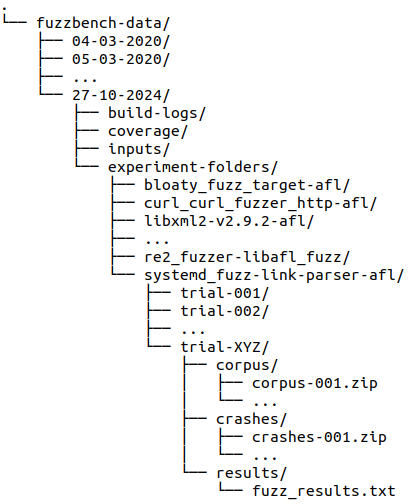
\includegraphics[scale=0.4]{foto/tree.png}
\caption{FuzzBench's Google Cloud directory tree}
\label{fig:tree}
\end{figure}
\ \\
All data on FuzzBench is grouped by test date, and each test set is composed by several key information:
\begin{itemize}
    \item \verb|build-logs|: contains the logs generated when building the fuzz targets
    \item \verb|coverage|: contains information related to the coverage achieved by each fuzzer on the different projects tested that day
    \item \verb|input|: contains the binaries executed to compile the different fuzz targets
    \item \verb|experiment-folders|: contains all the data related to the testing sessions
\end{itemize}

Following the experiments, each project has its own folder that specifies the name of the project, the fuzz target tested, the fuzzing engine used and sometimes also the objective of the session (bugs, coverage, correctness). Each project then undergoes several fuzzing sessions, identified by different \verb|trial| folders, providing all the information that were relevant to this work:
\begin{itemize}
    \item \verb|corpus|: contains several corpora stored as zip files.
    \item \verb|crashes|: contains all the crashes found in each trial as a separate zip file
    \item \verb|results|: contains the cumulative log of all fuzzing sessions
\end{itemize}


The objective of this analysis was to build the latest version of several experiments, download the content of all the available \verb|crashes| for each one of them and verify whether all these old crashes have been fixed or not.

Considering that downloading and analyzing the content of potentially tens of millions zip files would require several month, I was tasked with finding a way to differentiate between the different types of test sessions.
To do this, I found the \textit{experiment-requests.yaml} configuration file \cite{exp_yaml} inside the FuzzBench repository, which contained
all information related to the type of tests conducted, the projects tested as well as all the fuzzing engines used:

\begin{figure}[h]
\centering
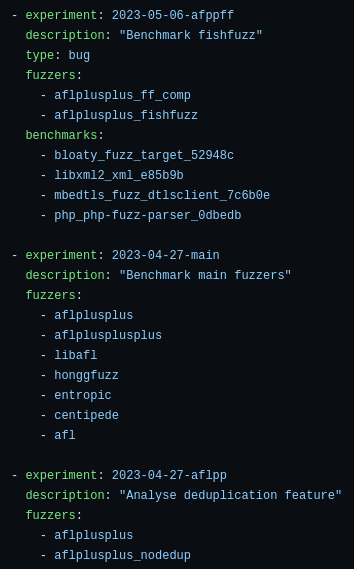
\includegraphics[scale=0.55]{foto/exp_yaml.png}
\caption{Excerpt fron the experiment configuration file}
\label{fig:exp_yaml}
\end{figure}
\ \\
Then, similarly to the process followed in section \ref{selection}, I wrote a simple Python script taking as input the above file and storing the name of all those experiments containing the string "type: bug".
However, this file only contained information on all experiments between 2020 and 2023, and unfortunately I was not able to find any reference on all the experiments performed in 2024, forcing me to analyze all of them.


Then, I was tasked with selecting the projects that will be analyzed.


Finally, to analyze all the experiments on FuzzBench GCB and download their content, I used the \textit{gsutil} suite provided by Google, which works similarly to the \verb|ls|, \verb|mv| and \verb|cp| command of the Linux shell, except that it takes as argument the url of a Gollge Cloud resource.

To retrieve all the resources needed, I wrote a Python script that essentially performs horizontal scraping over the directory tree shown in figure \ref{fig:tree}, storing at each intermediate steps the link of the next resource to list using the \verb|gsutil ls| command.
In conclusion, this analysis yielded 971656 zip file, for a total of (qualche milione di) crashes, and the following projects and harnesses being tested:

\noindent
\begin{tabularx}{\textwidth}{
    @{\hspace{2em}}% Space for left bullet
    >{\leavevmode\llap{\textbullet~}\raggedright\rule{0pt}{3ex}}% Left bullet + formatting of column
    X% Left column specification
    @{\quad\hspace{1em}}% Space between columns + right bullet space
    >{\leavevmode\llap{\textbullet~}\raggedright\arraybackslash}% Right bullet + formatting of column
    X% Right column specification
    @{}% No column space on right
  }
  arrow (parquet-arrow-fuzz) & aspell (aspell\_fuzzer) \\
  assimp (assimp\_fuzzer) & bloaty (fuzz\_target) \\
  curl (curl\_fuzzer\_http) & ffmpeg (ffmpeg\_demuxer\_fuzzer) \\
  file (magic\_fuzzer) & freetype2 (ftfuzzer) \\
  grok (grk\_decompress\_fuzzer) & harfbuzz (hb-shape-fuzzer) \\
  jsoncpp (jsoncpp\_fuzzer) & lcms (cms\_transform\_fuzzer) \\
  libaom (av1\_dec\_fuzzer) & libjpeg-turbo (libjpeg\_turbo\_fuzzer) \\
  libpcap (fuzz\_both) & libpng (libpng\_read\_fuzzer) \\
  libxml2 (xml) & mbedtls (fuzz\_dtlsclient) \\
  openssl (x509) & openthread (ot-ip6-send-fuzzer) \\
  php (php-fuzz-parser) & proj4 (proj\_crs\_to\_crs\_fuzzer) \\
  re2 (re2\_fuzzer) & sqlite3 (ossfuzz) \\
  systemd (fuzz-link-parser) & vorbis (decode\_fuzzer) \\
  woff2 (convert\_woff2ttf\_fuzzer) & zlib (zlib\_uncompress\_fuzzer)  
\end{tabularx}



\subsection{Testing with FuzzBench}
Explain how projects were built....
Explain how tests were automated and their duration...



\ziosaba{All the collected crashes were divided in 3 categories:
\begin{itemize}
    \item \textbf{crash:} inputs leading to any scenario that forces the system to close the process, like SEGV and heap/stack buffer overflows
    \item \textbf{out-of-memory (oom):} inputs inducing memory leaks or using huge allocation sizes to purposely test fail-safe mechanisms
    \item \textbf{timeout:} inputs that are either very long to parse or that purposely introduce unnecessary operations, again to test the resiliency of the program 
\end{itemize}}


When i testef fuzzbench and had to build using ASan + UBSan, i Didi this:
\begin{verbatim}
    $ docker run --rm --privileged 
        --platform linux/amd64 --memory=16g 
        -e PROJECT_NAME={project_name} -e HELPER=True 
        -e FUZZING_LANGUAGE=c++ -e FUZZING_ENGINE=afl 
        -e SANITIZER=address 
        -e SANITIZER_FLAGS_address="
            -fsanitize=address,array-bounds,bool,builtin,enum,
                integer-divide-by-zero,null,object-size,return,
                returns-nonnull-attribute,shift,
                signed-integer-overflow,unsigned-integer-overflow,
                unreachable,vla-bound,vptr
            -fno-sanitize-recover=array-bounds,bool,builtin,enum,
                integer-divide-by-zero,null,object-size,return,
                returns-nonnull-attribute,shift,
                signed-integer-overflow,unreachable,
                vla-bound,vptr 
            -fsanitize-address-use-after-scope" 
        -v /oss-fuzz/build/out/{project_name}/:/out/  
        -v /oss-fuzz/build/work/{project_name}/:/work/
        -v /oss-fuzz/build/corpus/{project_name}/:/corpus/
        -v /home/zio-saba/Scrivania/TESI/logfiles/:/logfiles/  
        -it  gcr.io/oss-fuzz/{project_name} /bin/bash
\end{verbatim}

